% ============================================================
% บทที่ 1: สถาปัตยกรรมและโพรโทคอลเครือข่าย Zigbee 3.0 สำหรับการเกษตรแม่นยำ
% ============================================================
\chapter[สถาปัตยกรรมและโพรโทคอลเครือข่าย Zigbee 3.0 สำหรับการเกษตรแม่นยำ]{สถาปัตยกรรมและโพรโทคอลเครือข่าย Zigbee 3.0\\สำหรับการเกษตรแม่นยำ}
\label{chap:ch01}

% ------------------------------------------------------------
% แผนบริหารการสอนประจำบทที่ 1 (หน้า 1/2)
% ------------------------------------------------------------
\section*{แผนบริหารการสอนประจำบทที่ 1}
\addcontentsline{toc}{section}{แผนบริหารการสอนประจำบทที่ 1}

\begin{planbox}{หัวข้อเนื้อหาประจำบท}
\begin{enumerate}[topsep=1pt, itemsep=0.5pt, partopsep=0pt, parsep=0pt, leftmargin=1.5em]
    \item รากฐานฟิสิกส์คลื่นวิทยุและการแพร่กระจายสัญญาณคลื่น 2.4 GHz ในทรงพุ่มแปลงเกษตร
    \item สถาปัตยกรรมและบทบาทของอุปกรณ์โครงข่ายตามมาตรฐาน Zigbee 3.0
    \item อัลกอริทึมการจัดเส้นทางแบบเมชและกลไกการซ่อมแซมโครงข่ายแบบพลวัต
    \item การวิเคราะห์เปรียบเทียบเชิงวิศวกรรมระหว่าง Zigbee 3.0, LoRaWAN, Wi-Fi และ BLE
    \item การออกแบบโครงสร้างโทโพโลยีแบบขยายขนาดได้สำหรับแปลงปลูกและโรงเรือนอัจฉริยะ
\end{enumerate}
\end{planbox}

\begin{planbox}{วัตถุประสงค์เชิงพฤติกรรม}
\begin{enumerate}[topsep=1pt, itemsep=0.5pt, partopsep=0pt, parsep=0pt, leftmargin=1.5em]
    \item อธิบายหลักการแพร่กระจายคลื่นและการสูญเสียกำลังส่งในแปลงเกษตรกรรมได้อย่างถูกต้อง
    \item จำแนกบทบาทและหน้าที่ของ Coordinator, Router และ End Device ได้อย่างแม่นยำ
    \item วิเคราะห์ขั้นตอนการค้นหาเส้นทางด้วยอัลกอริทึม AODV และการกู้คืนเครือข่ายได้
    \item เปรียบเทียบข้อได้เปรียบเชิงเทคนิคของระบบไร้สายแต่ละชนิดในงานฟาร์มอัจฉริยะได้
    \item ออกแบบแผนผังโครงข่ายแบบเมชรองรับพื้นที่แปลงเกษตรกรรมจริงได้อย่างมีประสิทธิภาพ
\end{enumerate}
\end{planbox}

\newpage

% ------------------------------------------------------------
% แผนบริหารการสอนประจำบทที่ 1 (หน้า 2/2)
% ------------------------------------------------------------
\begin{planbox}{วิธีสอนและกิจกรรมการเรียนการสอน}
\begin{enumerate}[topsep=1pt, itemsep=0.5pt, partopsep=0pt, parsep=0pt, leftmargin=1.5em]
    \item การบรรยายเชิงทฤษฎีควบคู่กับการยกตัวอย่างกรณีศึกษาแปลงเกษตรกรรมภาคตะวันออก
    \item การสาธิตการทำงานของโครงข่าย Zigbee Mesh ผ่านแบบจำลองและการดักจับแพ็กเก็ต
    \item การฝึกปฏิบัติการตรวจวัดความแรงสัญญาณ RSSI และ LQI ภายใต้สภาพแปลงปลูกจำลอง
    \item การจัดกิจกรรมกลุ่มเพื่อร่วมกันแก้โจทย์ปัญหาการเชื่อมต่อโหนดที่มีสิ่งกีดขวาง
    \item การมอบหมายงานศึกษาค้นคว้าอิสระและจัดทำรายงานวิเคราะห์โครงข่ายสื่อสาร
\end{enumerate}
\end{planbox}

\begin{planbox}{สื่อการเรียนการสอน}
\begin{enumerate}[topsep=1pt, itemsep=0.5pt, partopsep=0pt, parsep=0pt, leftmargin=1.5em]
    \item เอกสารประกอบการสอนวิชาสถาปัตยกรรมและโพรโทคอลเครือข่ายไร้สาย
    \item บอร์ดทดลองไมโครคอนโทรลเลอร์ CC2652P และ ESP32-C6 พร้อมเสาอากาศภายนอก
    \item ซอฟต์แวร์วิเคราะห์โครงข่าย Wireshark พร้อมอุปกรณ์ Zigbee Packet Sniffer
    \item วิดีทัศน์สาธิตการซ่อมแซมเส้นทางส่งสัญญาณเมื่อโหนดเราเตอร์หยุดทำงานกะทันหัน
    \item ผังโครงสร้างมาตรฐาน Zigbee Cluster Library และสเปกข้อกำหนดทางเทคนิค
\end{enumerate}
\end{planbox}

\begin{planbox}{การวัดและประเมินผล}
\begin{enumerate}[topsep=1pt, itemsep=0.5pt, partopsep=0pt, parsep=0pt, leftmargin=1.5em]
    \item การประเมินผลจากแบบทดสอบความรู้ก่อนเรียนและหลังเรียนประจำบท
    \item การประเมินทักษะการตั้งค่าอุปกรณ์และการดักจับแพ็กเก็ตในห้องปฏิบัติการ
    \item การประเมินคุณภาพรายงานการออกแบบโครงข่ายและการคำนวณงบประมาณการสูญเสียกำลัง
    \item การสังเกตพฤติกรรมการมีส่วนร่วมในการอภิปรายและการทำงานร่วมกันเป็นทีม
\end{enumerate}
\end{planbox}

\clearpage

% ------------------------------------------------------------
% เนื้อหาบทที่ 1
% ------------------------------------------------------------
\section{รากฐานฟิสิกส์คลื่นวิทยุและการลดทอนสัญญาณในแปลงเกษตรกรรม}

การส่งผ่านข้อมูลไร้สายในสภาพแวดล้อมทางการเกษตร \textbf{การแพร่กระจายคลื่นวิทยุ (Radio Frequency Propagation)}\index{Radio Propagation@Radio Propagation (การแพร่กระจายคลื่น)} ในย่านความถี่ ISM 2.4 GHz เผชิญกับความท้าทายทางกายภาพที่แตกต่างจากอาคารสำนักงานหรือพื้นที่โล่งทั่วไปอย่างสิ้นเชิง ทรงพุ่มใบพืช ลำต้น กิ่งก้าน ตลอดจนหยดน้ำค้างบนผิวใบ ล้วนมีพฤติกรรมเป็นตัวดูดกลืนและหักเหคลื่นแม่เหล็กไฟฟ้า ส่งผลให้คลื่นเกิดการลดทอนเชิงพื้นที่ (Path Loss)\index{Path Loss@Path Loss (การสูญเสียกำลังส่ง)} และการสะท้อนหลายเส้นทาง (Multipath Fading) อย่างมีนัยสำคัญ

การสูญเสียกำลังส่งในพื้นที่ว่าง (Free-Space Path Loss หรือ FSPL)\index{FSPL@FSPL (Free-Space Path Loss)} สำหรับคลื่นวิทยุที่มีความถี่ $f$ ในหน่วยเมกะเฮิร์ตซ์ และระยะทาง $d$ ในหน่วยกิโลเมตร สามารถคำนวณได้ตามแบบจำลองทางฟิสิกส์ดังสมการ
\begin{equation}
    \text{FSPL} = 20\log_{10}(d) + 20\log_{10}(f) + 32.44 \quad \text{[dB]}
\end{equation}

อย่างไรก็ดี ในแปลงปลูกพืชจริง ทรงพุ่มที่มีความหนาแน่นจะสร้างการลดทอนเพิ่มเติมตามแบบจำลอง \textbf{การลดทอนของฟิตซ์เจอรัลด์ (Modified Weissberger Model)} ซึ่งแสดงความสัมพันธ์ของการลดทอนจากใบพืช $L_{\text{veg}}$ ในหน่วยเดซิเบล สำหรับความลึกของทรงพุ่ม $d_f$ ในหน่วยเมตร ดังสมการ
\begin{equation}
    L_{\text{veg}} = 0.25 f^{0.39} d_f^{0.63} \quad \text{[dB]} \quad (14 < d_f \le 400)
\end{equation}
โดยที่ $f$ คือความถี่คลื่นในหน่วยกิกะเฮิร์ตซ์ ($f = 2.4$ GHz) จากสมการดังกล่าวจะเห็นได้ว่า เมื่อทรงพุ่มมีความหนาแน่นเพิ่มขึ้นในฤดูที่มีการผลิใบและติดผล สัญญาณคลื่นวิทยุจะลดทอนอย่างรวดเร็ว ส่งผลให้การเชื่อมต่อแบบจุดต่อจุดในระยะไกลไม่สามารถรักษาเสถียรภาพได้ การนำสถาปัตยกรรมโครงข่ายแบบเมชเข้ามาประยุกต์จึงเป็นทางเลือกเชิงวิศวกรรมที่มีประสิทธิภาพสูงสุด\index{Mesh Network@Mesh Network (โครงข่ายแบบเมช)}

\begin{figure}[H]
    \centering
    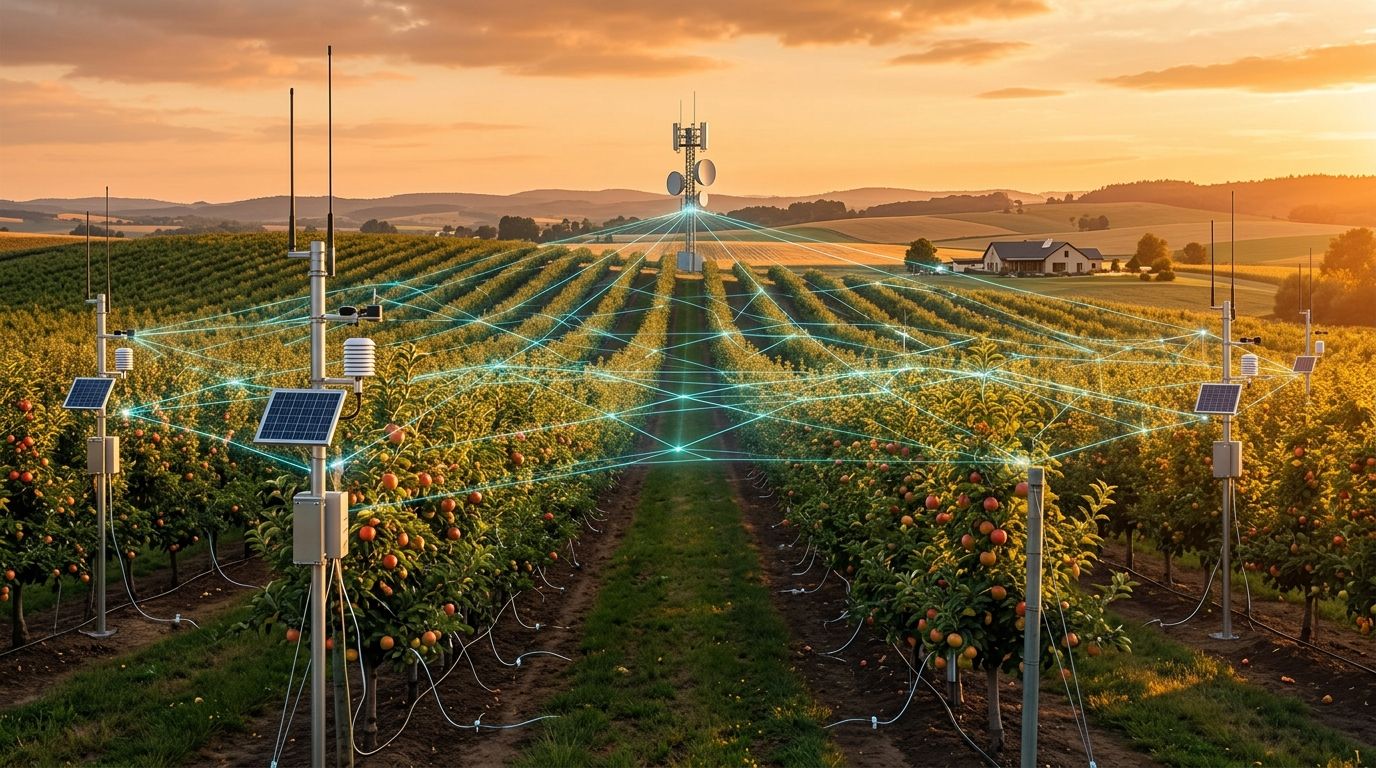
\includegraphics[width=0.92\textwidth]{figures/zigbee_farm_mesh_realistic.jpg}
    \caption{การติดตั้งโหนดโครงข่ายแบบเมช Zigbee 3.0 กระจายตัวในแปลงเกษตรกรรมและแปลงปลูกอัจฉริยะ}
    \label{fig:zigbee_farm_mesh}
\end{figure}

\section{สถาปัตยกรรมอุปกรณ์ตามมาตรฐาน Zigbee 3.0}

มาตรฐาน \textbf{ซิกบี 3.0 (Zigbee 3.0)}\index{Zigbee 3.0@Zigbee 3.0} ทำงานบนมาตรฐานชั้นกายภาพและชั้นควบคุมการเข้าถึงตัวกลาง IEEE 802.15.4\index{IEEE 802.15.4@IEEE 802.15.4} โดยผสานรวมมาตรฐานย่อยเดิม ได้แก่ Zigbee Home Automation, Zigbee Light Link และ Zigbee Building Automation เข้าไว้ด้วยกันภายใต้โปรไฟล์สากลหนึ่งเดียว ภายในเครือข่ายกำหนดบทบาทของอุปกรณ์ออกเป็น 3 ชนิด

\begin{protocolbox}[บทบาทและหน้าที่ของโหนดในเครือข่าย Zigbee 3.0]
โครงสร้างเครือข่ายแบ่งบทบาทของอุปกรณ์ตามการใช้พลังงานและหน้าที่ดังนี้
\begin{enumerate}
    \item \textbf{ตัวประสานงานเครือข่าย (Zigbee Coordinator หรือ ZC)}\index{Coordinator@Coordinator (ตัวประสานงาน)} เป็นโหนดหลักทำหน้าที่ริเริ่มเครือข่าย เลือกช่องสัญญาณความถี่ กำหนดค่าพารามิเตอร์ด้านความปลอดภัย จัดเก็บตารางการจัดเส้นทางระดับศูนย์กลาง และเชื่อมโยงสู่เกตเวย์ภายนอก ในเครือข่ายจะมี ZC ได้เพียง 1 ตัวเท่านั้น
    \item \textbf{เราเตอร์โครงข่าย (Zigbee Router หรือ ZR)}\index{Router@Router (เราเตอร์โครงข่าย)} ทำหน้าที่ส่งต่อแพ็กเก็ตข้อมูลระหว่างโหนด เป็นสะพานขยายระยะการส่งสัญญาณและทำหน้าที่รับคำขอเชื่อมต่อจากโหนดลูก อุปกรณ์เราเตอร์ต้องต่อไฟเลี้ยงตลอดเวลา
    \item \textbf{อุปกรณ์ปลายทาง (Zigbee End Device หรือ ZED)}\index{End Device@End Device (อุปกรณ์ปลายทาง)} เป็นโหนดตรวจวัดเซนเซอร์ที่ใช้พลังงานแบตเตอรี่ ไม่มีหน้าที่ส่งต่อข้อมูลให้โหนดอื่น และสามารถเข้าสู่โหมดประหยัดพลังงานระดับลึก (Deep Sleep) ได้นานหลายปี
\end{enumerate}
\end{protocolbox}

\begin{table}[H]
\caption{การเปรียบเทียบบทบาทและคุณลักษณะของโหนดในเครือข่าย Zigbee 3.0}
\label{tab:zigbee_device_roles}
\centering
\small
\begin{tabularx}{\textwidth}{p{3.2cm} >{\raggedright\arraybackslash}X >{\raggedright\arraybackslash}X c}
\toprule
\textbf{ชนิดอุปกรณ์} & \textbf{แหล่งจ่ายพลังงาน} & \textbf{บทบาทหลักในเครือข่าย} & \textbf{โหมดประหยัดไฟ} \\
\midrule
Coordinator (ZC) & ไฟฟ้ากระแสสลับต่อเนื่อง & ริเริ่มเครือข่าย, จัดการกุญแจความปลอดภัย & ไม่รองรับ \\
Router (ZR) & ไฟฟ้ากระแสสลับ หรือ โซลาร์ & ส่งต่อแพ็กเก็ตข้อมูล, ขยายรัศมีโครงข่าย & ไม่รองรับ \\
End Device (ZED) & แบตเตอรี่ Li-SOCl2 / LiFePO4 & อ่านค่าเซนเซอร์, ส่งข้อมูลขึ้นโหนดแม่ & รองรับ Deep Sleep \\
\bottomrule
\end{tabularx}
\end{table}

\section{อัลกอริทึมการจัดเส้นทางแบบเมชและการซ่อมแซมโครงข่ายด้วยตนเอง}

ความสามารถในการจัดเส้นทาง \textbf{การจัดเส้นทางแบบเมช (Mesh Routing)} ของ Zigbee อาศัยอัลกอริทึม AODV (Ad hoc On-Demand Distance Vector)\index{AODV Routing@AODV Routing (การจัดเส้นทาง)} ร่วมกับกลไกตารางเพื่อนบ้าน (Neighbor Table) เพื่อสร้างเส้นทางการส่งข้อมูลแบบหลายช่วง (Multi-hop) อัตโนมัติ

\begin{agribox}[กระบวนการค้นหาและซ่อมแซมเส้นทางอัตโนมัติ]
เมื่อโหนดเซนเซอร์ ZED หรือเราเตอร์ ZR ต้องการส่งข้อมูลไปยัง Coordinator กระบวนการทำงานเกิดขึ้นดังนี้
\begin{enumerate}
    \item \textbf{Route Request (RREQ)} โหนดต้นทางกระจายแพ็กเก็ตค้นหาเส้นทางไปยังเราเตอร์เพื่อนบ้านในระยะรัศมีคลื่นวิทยุ
    \item \textbf{Link Quality Assessment} เราเตอร์แต่ละตัวจะประเมินคุณภาพสัญญาณรับ (LQI) และค่าความแรงสัญญาณ (RSSI) เพื่อคำนวณต้นทุนการส่งผ่าน (Link Cost)
    \item \textbf{Route Reply (RREP)} โหนดปลายทางหรือเราเตอร์ที่มีเส้นทางสู่ปลายทาง จะส่งแพ็กเก็ตตอบกลับเพื่อยืนยันเส้นทางที่มีต้นทุนรวมต่ำที่สุด
    \item \textbf{Self-Healing Route Recovery}\index{Self-Healing@Self-Healing (การกู้คืนเครือข่าย)} หากเราเตอร์ตัวกลางหยุดทำงานเนื่องจากแบตเตอรี่หมดหรือถูกกีดขวาง โหนดต้นทางจะตรวจพบความล้มเหลวและเริ่มส่งแพ็กเก็ต RREQ ใหม่ เพื่อค้นหาเส้นทางสำรองรอบสิ่งกีดขวางภายในเวลาไม่กี่วินาที
\end{enumerate}
\end{agribox}

\section{การวิเคราะห์เปรียบเทียบระหว่าง Zigbee 3.0, LoRaWAN, Wi-Fi และ BLE}

ในการวางสถาปัตยกรรมระบบไอโอทีทางการเกษตร วิศวกรจำเป็นต้องเลือกเทคโนโลยีที่ตอบโจทย์ความต้องการของพื้นที่และปริมาณข้อมูลอย่างเหมาะสม\index{LoRaWAN@LoRaWAN} ตารางที่ \ref{tab:wireless_tech_comparison} สรุปเปรียบเทียบมาตรฐานสื่อสารสำคัญ

\begin{table}[H]
\caption{การวิเคราะห์เปรียบเทียบสมรรถนะเทคโนโลยีสื่อสารไร้สายในงานเกษตรกรรม}
\label{tab:wireless_tech_comparison}
\centering
\small
\begin{tabularx}{\textwidth}{p{2.6cm} c c c >{\raggedright\arraybackslash}X}
\toprule
\textbf{เทคโนโลยี} & \textbf{อัตราส่งข้อมูล} & \textbf{ระยะทางต่อช่วง} & \textbf{การใช้พลังงาน} & \textbf{จุดเด่นและความเหมาะสม} \\
\midrule
Zigbee 3.0 & 250 kbps & 30--100 m & ต่ำมาก (mA) & โครงข่ายเมชหลายโหนดหนาแน่น ค่า Latency ต่ำ \\
LoRaWAN & 0.3--50 kbps & 2--15 km & ต่ำมาก & โครงข่ายดาวระยะไกล เหมาะกับเซนเซอร์เดี่ยวห่างไกล \\
Wi-Fi (802.11b/g/n) & 11--150 Mbps & 50--100 m & สูง & แบนด์วิดท์สูง เหมาะสำหรับกล้องสตรีมภาพและวิดีโอ \\
BLE (Bluetooth 5) & 1--2 Mbps & 10--40 m & ต่ำมาก & ส่งข้อมูลระยะใกล้ เหมาะสำหรับการตั้งค่าหน้างาน \\
\bottomrule
\end{tabularx}
\end{table}

จากตารางข้างต้นจะเห็นได้ว่า สำหรับแปลงเกษตรกรรมแบบโรงเรือน แปลงผลไม้ที่มีการติดตั้งเซนเซอร์หนาแน่นหลายสิบโหนด และต้องการส่งข้อมูลแบบสองทิศทางเพื่อควบคุมวาล์วน้ำและสวิตช์อย่างทันท่วงที (Latency ไม่เกิน 100 มิลลิวินาที) เทคโนโลยี Zigbee 3.0 มีความได้เปรียบ LoRaWAN อย่างชัดเจนในแง่ของแบนด์วิดท์และความสามารถในการรับส่งคำสั่งควบคุม

\clearpage

% ------------------------------------------------------------
% คำถามทบทวนท้ายบทที่ 1
% ------------------------------------------------------------
\section*{คำถามทบทวนท้ายบทที่ 1}
\addcontentsline{toc}{section}{คำถามทบทวนท้ายบทที่ 1}

\begin{enumerate}
    \item จงอธิบายกลไกทางฟิสิกส์ที่ทำให้คลื่นความถี่ 2.4 GHz เกิดการสูญเสียกำลังส่งอย่างรวดเร็วเมื่อแพร่ผ่านทรงพุ่มแปลงผลไม้ พร้อมระบุตัวแปรสำคัญในแบบจำลองของฟิตซ์เจอรัลด์
    \item ในเครือข่าย Zigbee 3.0 เหตุใดจึงอนุญาตให้มี Coordinator ได้เพียง 1 ตัว และอุปกรณ์ชนิดใดบ้างที่สามารถทำหน้าที่ขยายรัศมีโครงข่ายแบบเมชได้
    \item อธิบายขั้นตอนการทำงานของอัลกอริทึม AODV เมื่อเกิดเหตุการณ์ที่เราเตอร์ตัวกลางหยุดทำงานกะทันหัน เครือข่ายมีกระบวนการซ่อมแซมเส้นทางด้วยตนเองอย่างไร
    \item จงเปรียบเทียบข้อดีและข้อจำกัดระหว่าง Zigbee 3.0 และ LoRaWAN ในการติดตั้งระบบน้ำอัจฉริยะที่ต้องการทั้งการอ่านค่าเซนเซอร์และการสั่งเปิดปิดโซลินอยด์วาล์ว 24 ตัว
    \item หากต้องการออกแบบเครือข่าย Zigbee สำหรับโรงเรือนอัจฉริยะขนาด 40 เมตรคูณ 100 เมตร จงระบุจำนวนและตำแหน่งที่เหมาะสมของ Coordinator, Router และ End Device เพื่อให้การเชื่อมต่อมีเสถียรภาพสูงสุด
\end{enumerate}

\clearpage
